\documentclass{article}
\usepackage{amsmath,amsthm,amssymb}
\usepackage[T1]{fontenc}
\usepackage[utf8]{inputenc}
\usepackage[english]{babel}
\usepackage{graphicx}
\usepackage{hyperref}
\usepackage{booktabs}
\usepackage{array}
\usepackage{tabularx}
\usepackage{tikz}
\usetikzlibrary{arrows.meta,positioning}

\title{Actionable Sales-Coaching Moment Detection}
\author{Evtushenko Vitaly}
\date{May 2026}

\begin{document}
\maketitle

\begin{abstract}
This study presents an applied NLP system for detecting actionable coaching moments in short English sales-dialogue fragments. The system receives a speaker-tagged dialogue window and predicts whether the fragment should be reviewed by a sales coach and whether it contains an unresolved customer concern. The final pipeline includes public dataset preparation, dialogue windowing, manual gold annotation, grouped cross-validation, classical text baselines, a transparent dialogue-structure rule, review-queue ranking, evidence extraction, confidence-based fallback behavior, and template recommendations. Project code is available at \url{https://github.com/Evtushenker/NLP2026_SalesCoachingMomentDetection}.
\end{abstract}

\section{Introduction}
Sales teams produce many customer conversations, but only a small part of them can be reviewed manually. A sales lead usually does not need a generic sentiment score for every call; they need to find concrete moments where a manager missed discovery, failed to resolve an objection, skipped the next step, or otherwise created a coaching opportunity. This makes the task naturally different from general text classification: the system should detect locally actionable fragments and present them in a form that a human reviewer can inspect.

This study frames the problem as a supervised NLP task over short dialogue windows. Each example is a local fragment with normalized speaker tags such as \texttt{manager} and \texttt{client}. The main output is a binary coaching-triage decision, supported by a second binary label for unresolved customer concerns. This formulation is useful because a manager can review the highest-priority windows instead of reading every transcript from beginning to end.

The main contribution is a reproducible review-oriented pipeline rather than a standalone classifier. The system combines manually reviewed gold labels, leakage-safe grouped evaluation by dialogue, interpretable baselines, prioritization metrics, copied evidence turns, and conservative recommendation templates. This differs from a black-box free-form coaching system: recommendations are grounded in extracted input evidence, and low-confidence examples fall back to manual review instead of receiving unsupported advice.

\subsection{Team}
\textbf{Evtushenko Vitaly} prepared the dataset, defined the labeling scheme, reviewed gold labels, implemented the baselines and evaluation scripts, and built the evidence and recommendation layer.

\section{Related Work}
\label{sec:related}
The work is connected to several established NLP directions.

\textbf{Dialogue act and intent classification.} Dialogue analysis often models utterances through their communicative function, for example whether a turn asks a question, provides information, confirms an action, or expresses a problem. This idea is close to the present project because sales-coaching moments depend on how manager and customer turns interact, not only on isolated word frequency. Standard dialogue-system surveys describe this broader setting and motivate structured treatment of conversational turns \cite{jurafskyMartin2024}.

\textbf{Classical text classification.} For datasets with limited gold annotation, TF-IDF features with linear classifiers remain strong baselines. They are transparent, fast, and less data-hungry than neural fine-tuning. The evaluation therefore uses scikit-learn implementations of Logistic Regression and Linear SVM as competitive classical baselines \cite{pedregosa2011scikit}. These baselines are appropriate for the current reviewed gold set of 100 windows.

\textbf{Sentence embeddings.} Sentence-level transformer embeddings provide a reusable representation for semantic similarity and classification. Sentence-BERT is a common approach for producing such embeddings efficiently \cite{reimers2019sentencebert}. Sentence-transformer embeddings are treated as an additional baseline rather than as the final system, because the reviewed gold set is focused and interpretability is important for review.

\textbf{Weak supervision and manual review.} Weak supervision can create training labels from heuristics and rules, but it can also overfit the behavior of those heuristics if final claims are not checked against manually reviewed data. Snorkel-style weak supervision motivates this distinction between noisy labeling functions and gold evaluation \cite{ratner2017snorkel}. Weak labels are used for development diagnostics, while final quality claims are based on manually reviewed windows.

\textbf{Conversation review and coaching tools.} Commercial conversation-intelligence systems usually rank or summarize calls for managers, but their internal labels and datasets are rarely public. Because there is no standard public benchmark for the exact ``actionable sales-coaching moment'' task used here, the evaluation compares transparent local baselines and reports practical review-queue metrics under the same protocol.

\section{Model Description}
\label{sec:model}
The proposed approach is a review pipeline for short sales-dialogue windows. It has five stages: transcript parsing, window construction, label prediction, evidence extraction, and recommendation generation. Figure~\ref{fig:pipeline} shows the complete flow.

\begin{figure}[!tbh]
    \centering
    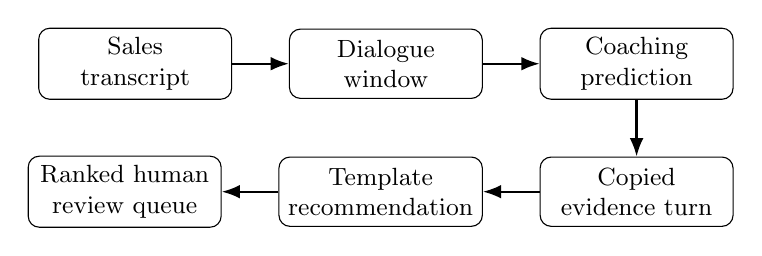
\begin{tikzpicture}[
        node distance=0.72cm,
        box/.style={draw, rounded corners, align=center, minimum width=2.45cm, minimum height=0.88cm, font=\small},
        arrow/.style={-Latex, thick}
    ]
        \node[box] (transcript) {Sales\\transcript};
        \node[box, right=of transcript] (window) {Dialogue\\window};
        \node[box, right=of window] (prediction) {Coaching\\prediction};
        \node[box, below=of prediction] (evidence) {Copied\\evidence turn};
        \node[box, left=of evidence] (recommendation) {Template\\recommendation};
        \node[box, left=of recommendation] (queue) {Ranked human\\review queue};

        \draw[arrow] (transcript) -- (window);
        \draw[arrow] (window) -- (prediction);
        \draw[arrow] (prediction) -- (evidence);
        \draw[arrow] (evidence) -- (recommendation);
        \draw[arrow] (recommendation) -- (queue);
    \end{tikzpicture}
    \caption{Final sales-coaching review pipeline. The model does not only predict labels; it also ranks windows, extracts copied evidence, and produces conservative recommendations for human review.}
    \label{fig:pipeline}
\end{figure}

\subsection{Input Representation}
Each transcript is parsed into ordered speaker turns. The system normalizes speakers into two roles, \texttt{manager} and \texttt{client}, and builds overlapping dialogue windows. The default window contains 4 turns with stride 2. A typical input has the following form:
\begin{verbatim}
manager: ...
client: ...
manager: ...
client: ...
\end{verbatim}

The 4-turn window is used because it usually contains both a customer signal and the manager response or non-response. Shorter windows can miss context, while longer windows can mix several coaching moments.

\subsection{Prediction Targets}
The final system focuses on two binary targets:
\begin{itemize}
    \item \texttt{actionable\_coaching\_needed}: the fragment contains a concrete moment that deserves sales-coach review;
    \item \texttt{unresolved\_customer\_concern}: the customer expresses a concern or objection that is still open inside the visible context.
\end{itemize}

Auxiliary labels are kept for explanation and recommendations: \texttt{needs\_discovery}, \texttt{value\_articulation}, \texttt{objection\_handling}, \texttt{next\_step\_fixed}, and \texttt{early\_presentation\_before\_discovery}. They are not all equally suitable for final modeling because some labels are rare in the reviewed sample.

\subsection{Open-Concern Rule}
The strongest unresolved-concern approach is a transparent dialogue-structure rule. It checks whether the latest client turn contains concern language and whether there is no later manager turn resolving it. For a window $w$, the rule can be written as:
\[
\text{open\_concern}(w)=
\mathbb{1}[\exists c_{\text{last}} \in w:
c_{\text{last}} \text{ matches concern pattern}
\land \neg \exists m \text{ after } c_{\text{last}}].
\]
This rule is intentionally simple. It captures the local structure of an unresolved objection and is easy to audit when it flags an example.

\subsection{Evidence and Recommendation Layer}
For flagged windows, the system extracts the input turn that explains the prediction. For unresolved concerns, this is the latest client concern that remains unanswered in the window. The evidence is copied from the input text; the system does not invent supporting facts.

The final recommendation is template-based. High-confidence examples receive a direct but generic coaching action, medium-confidence examples are marked for review, and low-confidence examples return a manual-review fallback. This design keeps the output useful while avoiding unsupported free-form advice.

\section{Dataset}
This study uses the public Hugging Face dataset \texttt{gwenshap/sales-transcripts} \cite{gwenshapSalesTranscripts}. The dataset contains English synthetic sales conversation transcripts and is distributed under the Apache-2.0 license. It can be obtained from \url{https://huggingface.co/datasets/gwenshap/sales-transcripts}. The data is suitable for studying sales-dialogue coaching signals because it is public, conversation-level, and licensed for reuse.

The original dataset is not provided as a ready-made benchmark for the exact task considered here. Therefore, the data was transformed into the target evaluation format through the following preprocessing and annotation procedure:
\begin{enumerate}
    \item download public transcript files from the dataset;
    \item parse each transcript into ordered speaker turns;
    \item normalize speaker roles to \texttt{manager} and \texttt{client};
    \item build overlapping 4-turn windows with stride 2;
    \item create weak labels for exploratory development;
    \item manually review a 100-window sample and derive focused binary targets.
\end{enumerate}

Table~\ref{tab:data-stats} gives the main dataset statistics used in the report.

\begin{table}[!tbh]
    \centering
    \begin{tabular}{lrp{0.42\linewidth}}
        \toprule
        Artifact & Count & Description \\
        \midrule
        Source transcripts & 50 & Public synthetic sales dialogues from Hugging Face \\
        Candidate windows & 427 & 4-turn windows with stride 2 \\
        Gold-reviewed windows & 100 & Manual review subset used for final evaluation \\
        Dialogue groups in gold set & 12 & Used as groups in cross-validation \\
        Actionable coaching positives & 59 & Positive examples for the main coaching-triage task \\
        Unresolved concern positives & 39 & Positive examples for the open-customer-concern task \\
        \bottomrule
    \end{tabular}
    \caption{Dataset statistics after preprocessing and manual review.}
    \label{tab:data-stats}
\end{table}

The weak-label development split is grouped by dialogue: 35 train dialogues, 7 validation dialogues, and 8 test dialogues. The final reported evaluation does not use this split for quality claims; it uses grouped cross-validation on the 100 manually reviewed windows. Grouping by \texttt{dialogue\_id} prevents windows from the same transcript from appearing in both train and test folds.

Table~\ref{tab:aux-labels} shows the auxiliary gold-label distribution. The rare class \texttt{early\_presentation\_before\_discovery} has only 2 positive examples, so it is not treated as a reliable final supervised target.

\begin{table}[!tbh]
    \centering
    \begin{tabular}{lrr}
        \toprule
        Label & Positive & Negative \\
        \midrule
        \texttt{needs\_discovery} & 54 & 46 \\
        \texttt{value\_articulation} & 67 & 33 \\
        \texttt{objection\_handling} & 44 & 56 \\
        \texttt{next\_step\_fixed} & 21 & 79 \\
        \texttt{early\_presentation\_before\_discovery} & 2 & 98 \\
        \bottomrule
    \end{tabular}
    \caption{Auxiliary label distribution on the 100 manually reviewed windows.}
    \label{tab:aux-labels}
\end{table}

\section{Experiments}
\subsection{Metrics}
The main classification metrics are precision, recall, and F1:
\[
\text{Precision}=\frac{TP}{TP+FP},\quad
\text{Recall}=\frac{TP}{TP+FN},\quad
F_1=\frac{2PR}{P+R}.
\]

Because the practical use case is human review prioritization, the evaluation also reports Average Precision and top-$k$ review metrics. For a review budget of $k$ windows:
\[
\text{lift@}k = \frac{\text{precision@}k}{\text{positive rate}}.
\]
Lift shows how much better the ranked queue is than random review under the same budget.

The evidence layer is evaluated separately: extracted evidence should be copied from the input window and should explain the flag. The confidence layer is checked by verifying that low-confidence examples use fallback behavior and do not receive specific coaching advice.

\subsection{Experiment Setup}
The final focused-task experiment uses 5-fold grouped cross-validation over the 100 manually reviewed windows. The group key is \texttt{dialogue\_id}. This is important because adjacent windows from the same transcript are similar; a random row split would overestimate quality.

The classical trainable models use TF-IDF features over the window text. Logistic Regression uses class balancing and a linear decision boundary. Linear SVM is included as a second strong sparse-text baseline. The sentence-embedding baseline uses \texttt{all-MiniLM-L6-v2} embeddings with Logistic Regression. The transparent open-concern rule has no trainable parameters and is evaluated directly on each fold's held-out rows.

For review-queue evaluation, out-of-fold predictions from the grouped cross-validation are sorted by model score. The top-20\% budget corresponds to 20 windows out of the 100-window gold sample.

\subsection{Baselines}
The final approach is compared against the following baselines:
\begin{itemize}
    \item \textbf{Majority baseline}: always predicts the majority class and shows how much class imbalance alone can explain.
    \item \textbf{Rule baseline}: uses transparent patterns for open concerns and next-step signals.
    \item \textbf{TF-IDF + Logistic Regression}: a strong sparse-text classifier for limited gold annotation.
    \item \textbf{TF-IDF + Linear SVM}: another standard linear classifier for text classification.
    \item \textbf{Sentence embeddings + Logistic Regression}: a semantic embedding baseline using a pretrained sentence-transformer encoder.
\end{itemize}

There is no public previous-art leaderboard for this exact coaching-window task and dataset combination. Therefore, the most meaningful comparison is between transparent local baselines under the same grouped evaluation protocol.

\section{Results}
\subsection{Focused Task Results}
Table~\ref{tab:focused-results} reports the main grouped-CV comparison. The best practical model depends on the target. For \texttt{actionable\_coaching\_needed}, TF-IDF + Logistic Regression gives the strongest F1. For \texttt{unresolved\_customer\_concern}, the transparent open-concern rule outperforms the trainable text models.

\begin{table}[!tbh]
    \centering
    \begin{tabular}{llrrrr}
        \toprule
        Target & Model & F1 & F1 std & Precision & Recall \\
        \midrule
        unresolved concern & open-concern rule & 0.810 & 0.076 & 0.820 & 0.809 \\
        unresolved concern & TF-IDF + LogReg & 0.715 & 0.078 & 0.665 & 0.784 \\
        unresolved concern & TF-IDF + SVM & 0.664 & 0.077 & 0.662 & 0.686 \\
        actionable coaching & majority & 0.736 & 0.062 & 0.587 & 1.000 \\
        actionable coaching & open-concern / next-step rule & 0.761 & 0.058 & 0.850 & 0.707 \\
        actionable coaching & TF-IDF + LogReg & 0.862 & 0.059 & 0.781 & 0.965 \\
        actionable coaching & TF-IDF + SVM & 0.861 & 0.038 & 0.794 & 0.949 \\
        \bottomrule
    \end{tabular}
    \caption{Focused binary task results with 5-fold grouped cross-validation.}
    \label{tab:focused-results}
\end{table}

The result suggests that broad coaching triage benefits from learned lexical features, while unresolved concern detection is mostly a local dialogue-structure problem in the current dataset. This is why the final system keeps both a trainable model and an interpretable rule.

\subsection{Review-Queue Results}
Table~\ref{tab:queue-results} evaluates the models as ranking tools for human review. This is the most relevant practical metric because a sales lead usually reviews only a limited number of fragments.

\begin{table}[!tbh]
    \centering
    \begin{tabular}{llrrrr}
        \toprule
        Target & Ranking model & AP & Top-20 P & Top-20 R & Lift \\
        \midrule
        actionable coaching & TF-IDF + LogReg & 0.847 & 0.950 & 0.322 & 1.610 \\
        unresolved concern & open-concern rule & 0.792 & 0.900 & 0.462 & 2.308 \\
        \bottomrule
    \end{tabular}
    \caption{Best review-queue results from out-of-fold predictions.}
    \label{tab:queue-results}
\end{table}

At a top-20\% review budget, the actionable-coaching queue contains 19 positive windows out of 20. The unresolved-concern queue contains 18 positive windows out of 20. This confirms that the pipeline is useful as a triage tool on the current reviewed sample.

\subsection{Window-Size Ablation}
Table~\ref{tab:window-ablation} compares 2-turn, 4-turn, and 6-turn anchored variants of the same reviewed examples. Labels for 2-turn and 6-turn variants are projected from the original 4-turn gold labels, so this experiment is a robustness check rather than a new annotation study.

\begin{table}[!tbh]
    \centering
    \begin{tabular}{rllrrr}
        \toprule
        Turns & Target & Best model & F1 & Precision & Recall \\
        \midrule
        2 & unresolved concern & open-concern rule & 0.810 & 0.820 & 0.809 \\
        4 & unresolved concern & open-concern rule & 0.810 & 0.820 & 0.809 \\
        6 & unresolved concern & TF-IDF + LogReg & 0.751 & 0.696 & 0.824 \\
        2 & actionable coaching & TF-IDF + LogReg & 0.849 & 0.812 & 0.910 \\
        4 & actionable coaching & TF-IDF + LogReg & 0.862 & 0.781 & 0.965 \\
        6 & actionable coaching & TF-IDF + LogReg & 0.873 & 0.811 & 0.953 \\
        \bottomrule
    \end{tabular}
    \caption{Window-size ablation with projected labels.}
    \label{tab:window-ablation}
\end{table}

The 4-turn setup remains the default because it preserves the manually reviewed unit, keeps the open-concern rule strong, and gives high review-queue precision.

\subsection{Evidence, Confidence, and Inference Example}
Evidence extraction was evaluated on 30 predicted-positive unresolved-concern examples from the open-concern rule. All 30 extracted evidence turns were copied from the input window. The fallback count was 0. Among these 30 examples, 26 were gold-positive; the remaining 4 were prediction false positives rather than evidence-copy failures.

The integrated confidence demo contains 30 examples: 12 high-confidence rows, 12 medium-confidence rows, and 6 low-confidence rows. All 6 low-confidence rows use the \texttt{manual\_review} fallback, and no low-confidence example receives specific coaching advice.

Table~\ref{tab:output} shows one representative inference output.

\begin{table}[!tbh]
    \centering
    \begin{tabularx}{0.96\linewidth}{>{\raggedright\arraybackslash}X}
        \toprule
        \textbf{Input window:} \newline
        manager: I understand you've been browsing our online store. Is there anything specific you're looking for today? \newline
        client: Well, I've been looking at some winter jackets, but I'm not sure about the quality and if they're worth the price. \\
        \midrule
        \textbf{Prediction:} \texttt{unresolved\_customer\_concern = 1}; model: open-concern rule; score: 1.0. \\
        \midrule
        \textbf{Evidence:} client: Well, I've been looking at some winter jackets, but I'm not sure about the quality and if they're worth the price. \\
        \midrule
        \textbf{Recommendation:} Address the customer's latest concern before moving on: restate it, answer with a specific fact or policy, and check whether it is resolved. \\
        \bottomrule
    \end{tabularx}
    \caption{Example output from the evidence and recommendation layer.}
    \label{tab:output}
\end{table}

\subsection{Error Analysis}
The main observed error patterns are:
\begin{itemize}
    \item \texttt{needs\_discovery}: models over-predict discovery when a manager asks generic support questions.
    \item \texttt{value\_articulation}: indirect value statements are sometimes missed.
    \item \texttt{objection\_handling}: models miss handled objections because the task requires matching a customer concern with a manager response.
    \item \texttt{next\_step\_fixed}: models over-predict concrete next steps on soft closing phrases such as ``feel free to reach out''.
    \item \texttt{early\_presentation\_before\_discovery}: the class is too rare in the gold sample for reliable supervised learning.
\end{itemize}

\section{Conclusion}
The study prepared a public synthetic sales-dialogue dataset for an actionable coaching-window task, created a manually reviewed 100-window gold sample, implemented classical and rule-based baselines, evaluated them with grouped cross-validation, and added a practical review layer with ranking, evidence extraction, confidence handling, and template recommendations.

The best focused-task results are F1 0.862 for \texttt{actionable\_coaching\_needed} with TF-IDF + Logistic Regression and F1 0.810 for \texttt{unresolved\_customer\_concern} with a transparent open-concern rule. In the review-queue setting, the top 20\% highest-priority windows reach precision 0.950 for actionable coaching and 0.900 for unresolved customer concerns.

The main limitations are the current manually reviewed sample size, the lack of independent double annotation, and the synthetic nature of the source data. Future work should add more gold-labeled windows, measure inter-annotator agreement, and validate the approach on anonymized real sales conversations.

\begin{thebibliography}{9}

\bibitem{gwenshapSalesTranscripts}
gwenshap.
\newblock Sales Transcripts Dataset.
\newblock Hugging Face dataset, Apache-2.0 license.
\newblock \url{https://huggingface.co/datasets/gwenshap/sales-transcripts}.

\bibitem{jurafskyMartin2024}
Daniel Jurafsky and James H. Martin.
\newblock Speech and Language Processing.
\newblock Draft, 3rd edition, 2024.
\newblock \url{https://web.stanford.edu/~jurafsky/slp3/}.

\bibitem{pedregosa2011scikit}
Fabian Pedregosa, Gael Varoquaux, Alexandre Gramfort, Vincent Michel, Bertrand Thirion, Olivier Grisel, Mathieu Blondel, Peter Prettenhofer, Ron Weiss, Vincent Dubourg, Jake Vanderplas, Alexandre Passos, David Cournapeau, Matthieu Brucher, Matthieu Perrot, and Edouard Duchesnay.
\newblock Scikit-learn: Machine Learning in Python.
\newblock \emph{Journal of Machine Learning Research}, 12:2825--2830, 2011.

\bibitem{ratner2017snorkel}
Alexander Ratner, Stephen H. Bach, Henry Ehrenberg, Jason Fries, Sen Wu, and Christopher Re.
\newblock Snorkel: Rapid Training Data Creation with Weak Supervision.
\newblock \emph{Proceedings of the VLDB Endowment}, 11(3):269--282, 2017.

\bibitem{reimers2019sentencebert}
Nils Reimers and Iryna Gurevych.
\newblock Sentence-BERT: Sentence Embeddings using Siamese BERT-Networks.
\newblock In \emph{Proceedings of the 2019 Conference on Empirical Methods in Natural Language Processing}, pages 3982--3992, 2019.

\end{thebibliography}

\end{document}
